\documentclass{article}
\usepackage{amsmath}
\usepackage{fancyhdr}
\usepackage{amsmath}
\usepackage{clrscode}
\usepackage{subfigure}
\usepackage[top=3cm, bottom=3cm, left=3cm, right=3cm]{geometry}
\usepackage[pdftex]{graphicx}\title{BME511L: EEG Model Details}
\usepackage{float}
\usepackage{amsfonts}
\author{Allen Yin}
\pagestyle{fancy}
\setlength\parindent{0.0in}
\setlength\parskip{0.0in}
\usepackage{caption}
\captionsetup{justification=justified}
\setcounter{tocdepth}{2}
\setlength{\headheight}{15pt}

\begin{document}
\maketitle
\setlength\parskip{0.1in}

The brain consists of about $10^{10}$ neurons, with varying shape, size, and orientations. Invidivudal neurons can generate a small amount of electrical activity, which cannot be picked up by surface electrodes on the scalp. However, when a large group of neurons is simultaneously activated, the resulting electrical activity is large enough to be picked up by the electrodes at the surface, generating the Electroencephalography (EEG).


\section{Introduction}
For my project, I plan to use four dipoles inside a three concentric-shell spherical head model to model the sources of EEG signals. The locations of the dipoles will be fixed within the spherical model but their dipole moments will be time-dependent. These dipole moments will be calculated using the Reciprocity Principle to generate EEG waveforms at five electrode locations to match those obtained in a real experiment.

Then I will conduct sensitivity analysis on how these calculated dipole moments will change given more noisy EEG measurements at the electrodes.

\section{Model Details}

\subsection{Head Model}
The head model used will be the three concentric spherical shell model, whose cross section is shown in Figure 1. \cite{RushDriscoll1} has shown that this model of the head is a useful representation for many purposes. \cite{RushDriscoll2} compared the data from the model to ''electrolytic tank measurements employing a human skull, to in vivo data from within a monkey brain, and to in nivo data taken from the surface of the head [and found] with some minor exceptions\ldots the correlations are such as to indicate clearly that the model has adequate accuracy for most purposes presently forseen''.

\begin{figure}
    \begin{center}
        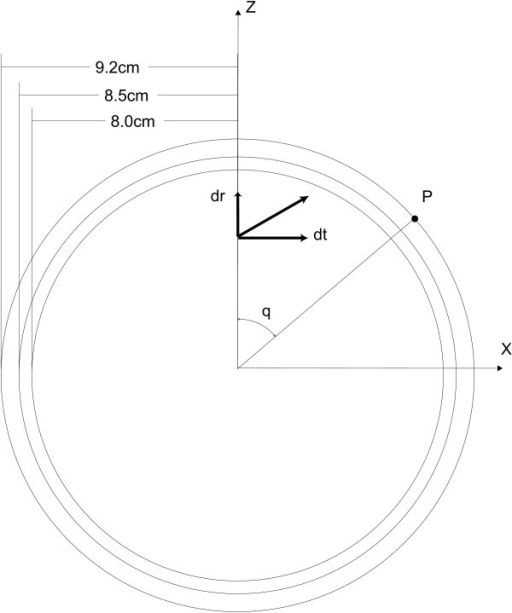
\includegraphics[scale=0.3]{concentric_shells.png}
        \caption{Cross section of the concentric shells head model. The shells from inside to outside represent the brain, skull, and scalp, respectively.}
    \end{center}
\end{figure}

The parameters for the head models are:
\begin{itemize}
    \item Brain: radius=$8.0cm$, resisitivity=$222\Omega\cdot cm$.
    \item Skull: radius=$8.5cm$, resisitivity=$80*222\Omega\cdot cm=17.76k\Omega\cdot cm$.
    \item Scalp: radius=$9.2cm$, resisitivity=$222\Omega\cdot cm$.
\end{itemize}

\subsection{Dipole Sources}
The generators of the EEG potential in my model will be 4 dipoles. I chose 4 because \cite{3dipole} has shown that 3 dipoles were able to explain $90\%$ of the observed potentials measured at the EEG electrodes in its experiment. As shown in Figure 2, I have fixed the dipole sources within the brain-tissue (sphere of radius=$8cm$). The sources are evenly distribued in the y-z plane. In other words, the azimuth angle of the sources are 0. The Cartesian coordinates of the dipole sources are: $(0,4,4)$, $(0,4,-4)$, $(0,-4,4)$, and $(0,-4,-4)$.

\begin{figure}
    \begin{center}
        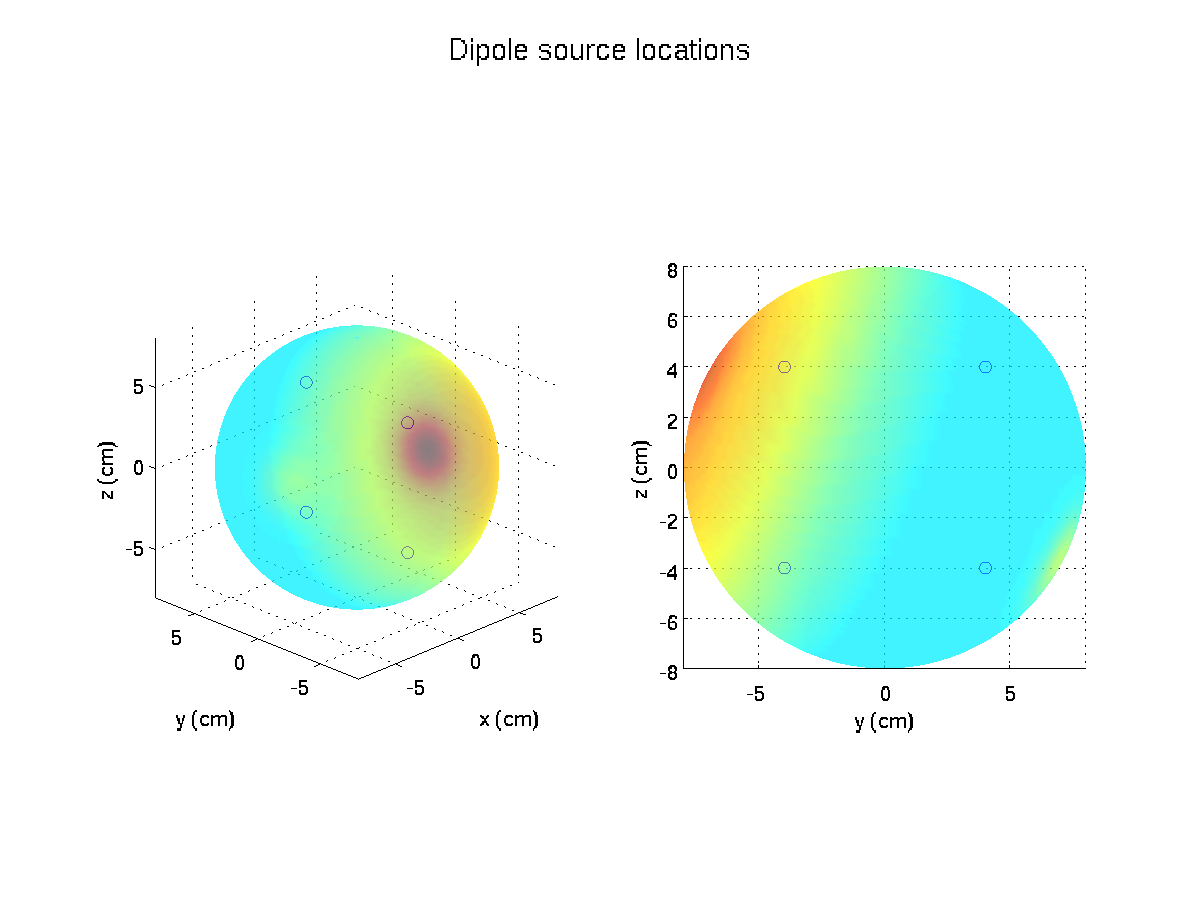
\includegraphics[scale=0.5]{dipole_sources.png}
        \caption{Left: 3D illustration of the dipole locations; Right: The dipole sources are evenly distributed in the y-z plane}.
    \end{center}
\end{figure}

\subsection{Electrodes and Expected EEG Waveforms}
The goal of the project is to determine the time-evolution of the four dipole sources needed to generate the EEG signals observed at the surface electrodes on the scalp. Since there are four dipole sources, there are 8 unknowns, therefore measurements at at least 5 electrodes are needed to solve this problem (4 electrodes provide only at most 6 equations).

I have chosen 5 electrode locations from the 10-20 system for EEG recording: \emph{Cz}, \emph{Fz}, \emph{Pz}, \emph{C3}, and \emph{C4}. Figure 3 shows the electrode locations looking down at the top of the head. The Figure is generated from the EEGLab\cite{EEGLab}. The Cartesian coordinates of the electrode locations are:
\begin{itemize}
    \item Fz: $R_{scalp}*(0.715,0,0.700)$.
    \item Cz: $R_{scalp}*(0,0,1)$.
    \item Pz: $R_{scalp}*(-0.715,0,0.700)$.
    \item C3: $R_{scalp}*(0,0.743,0.699)$.
    \item C4: $R_{scalp}*(0,-0.743,0.699)$.
\end{itemize}
, where $R_{scalp}$ is the radius of the outermost shell.

\begin{figure}
    \begin{center}
        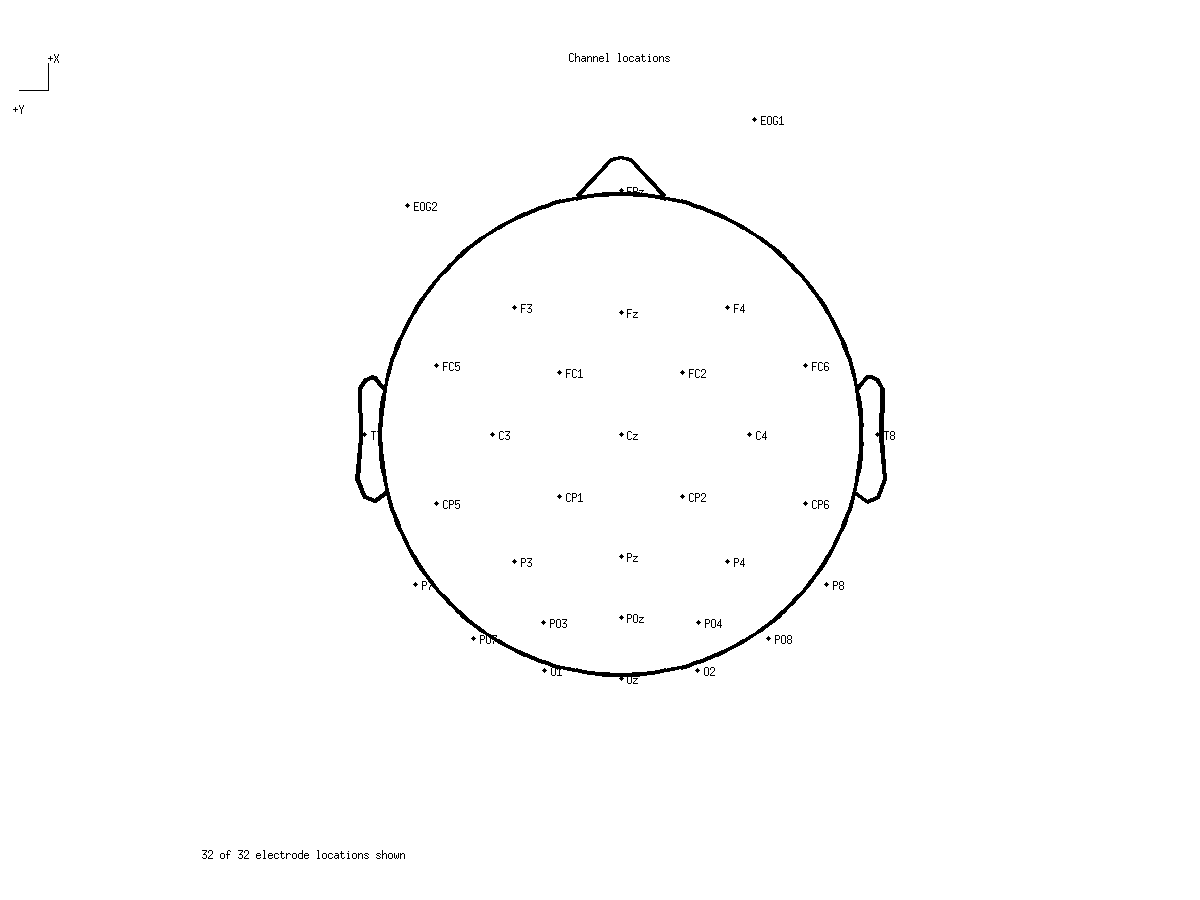
\includegraphics[scale=0.5]{channel_locations.png}
        \caption{The 10-20 system for EEG electrode placements. The electrodes used in this model are \emph{Cz}, \emph{Fz}, \emph{Pz}, \emph{C3}, and \emph{C4}}.
    \end{center}
\end{figure}

The expected EEG waveform is obtained from the sample dataset that came with the EEGLab software\cite{EEGLab}. The dataset was from the experiments conducted in \cite{EEGSource}. In the experiment, subjects were to focus at one of five target locations along a horizontal line. Whenever a square appeared in that target location, the subject responds by pressing a button. Any other stimulus such as a circle appearing in the target location, or a square appearing in other locations should be ignored. During each trial, the event-related potentials (ERPs) were recorded.

The sample dataset includes 80 such trials for one subjects, 40 trials for target location 1, and 40 for target location 2. For my model, I will average the ERPs at my specified electrodes over all 80 trials, and calculate the time evolution of the source dipoles to obtain those waveforms. Figure 4-8 shows the expected waveforms.

\begin{figure}
    \begin{center}
        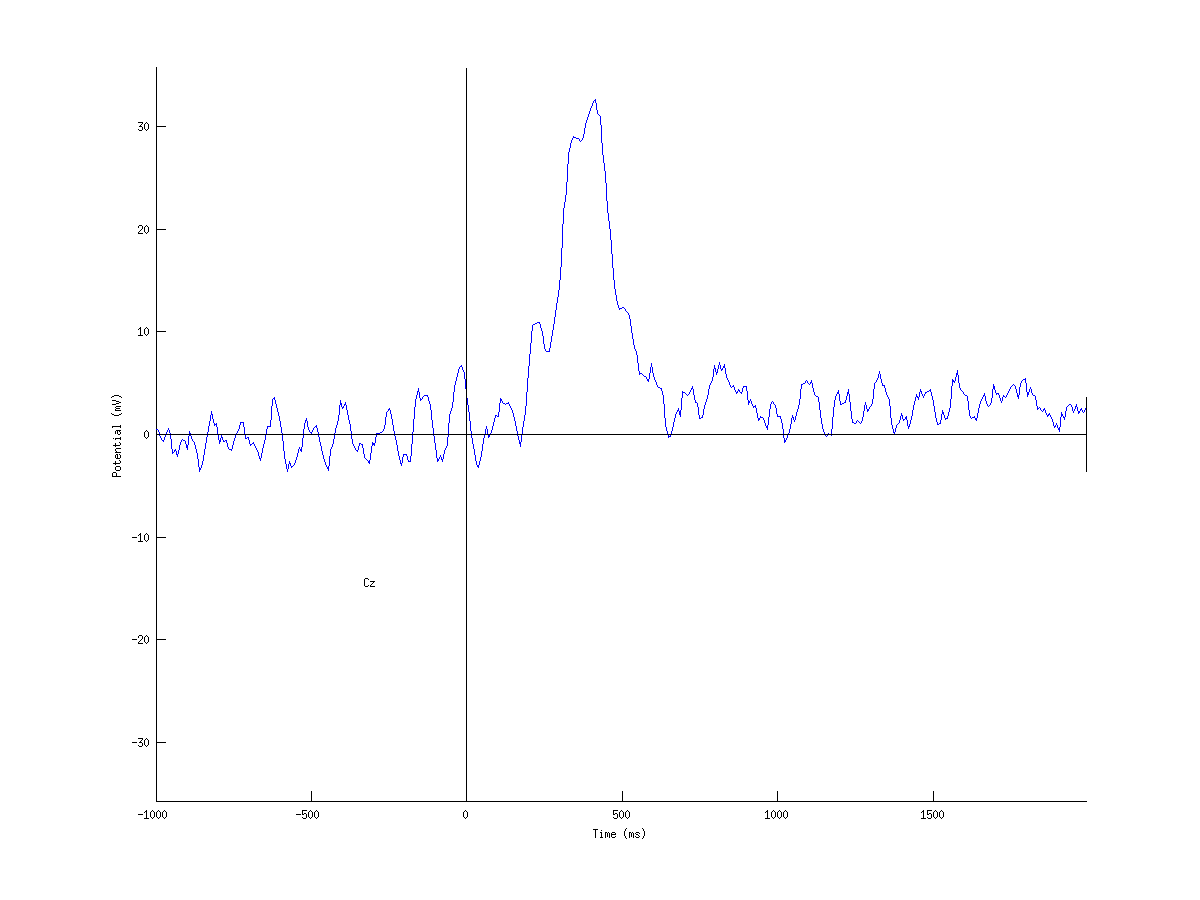
\includegraphics[scale=0.5]{Cz.png}
        \caption{Expected waveform for \emph{Cz}}
    \end{center}
\end{figure}
\begin{figure}
    \begin{center}
        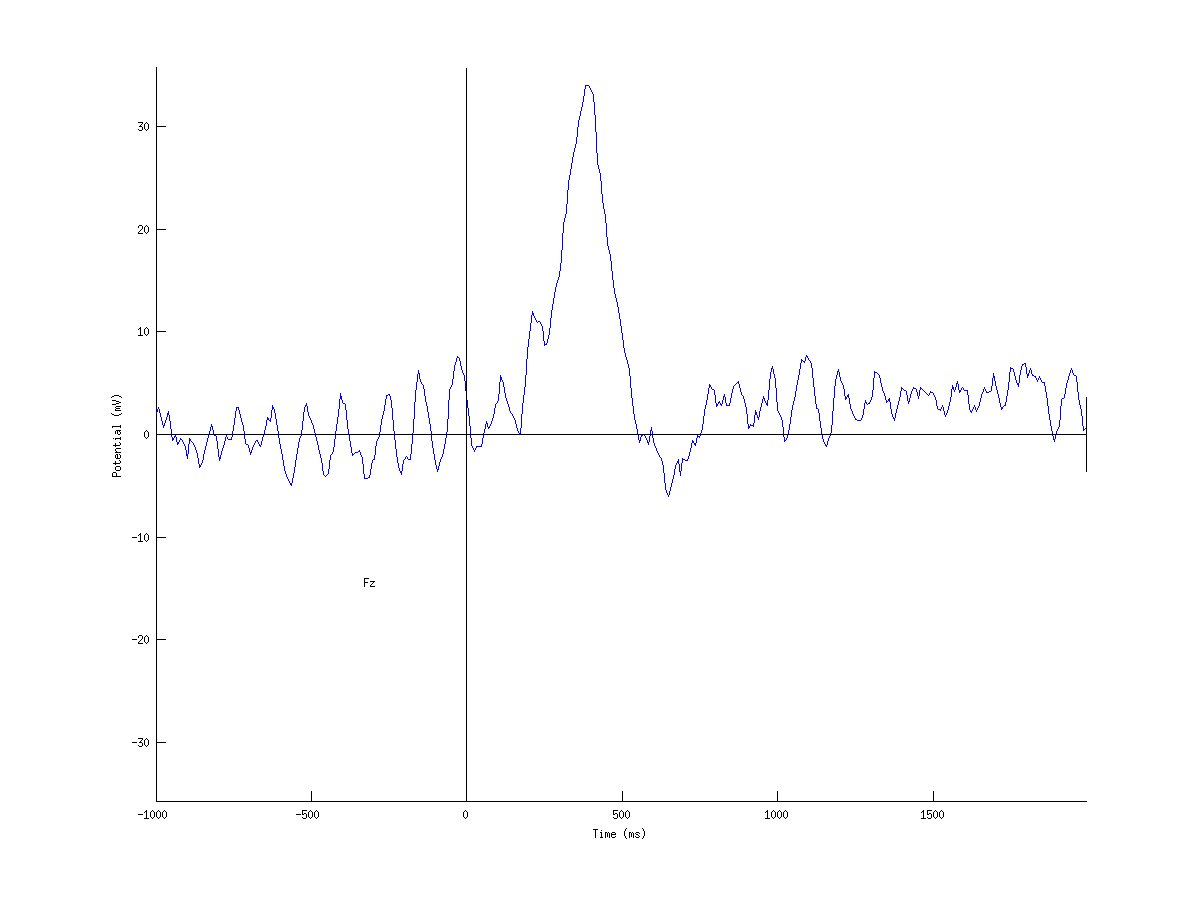
\includegraphics[scale=0.5]{Fz.png}
        \caption{Expected waveform for \emph{Fz}}
    \end{center}
\end{figure}
\begin{figure}
    \begin{center}
        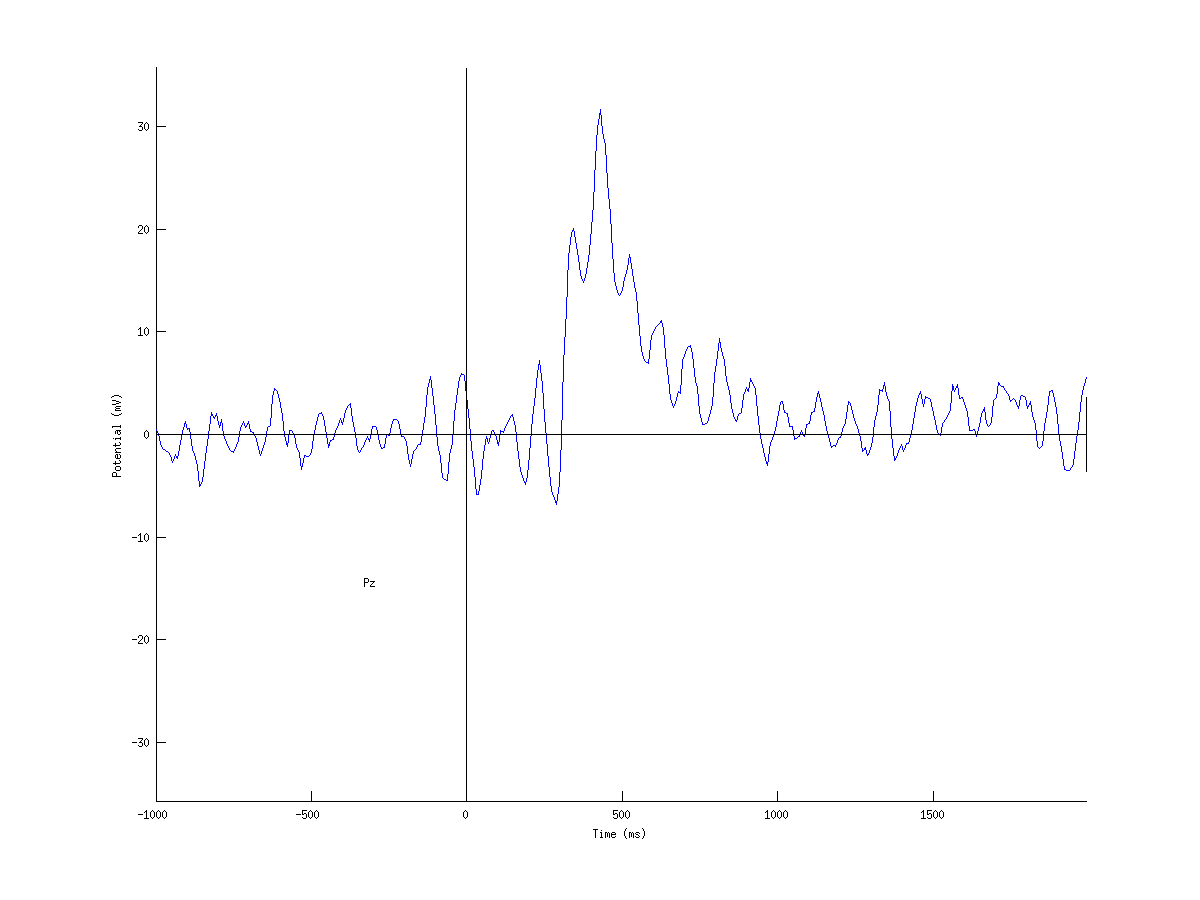
\includegraphics[scale=0.5]{Pz.png}
        \caption{Expected waveform for \emph{Pz}}
    \end{center}
\end{figure}
\begin{figure}
    \begin{center}
        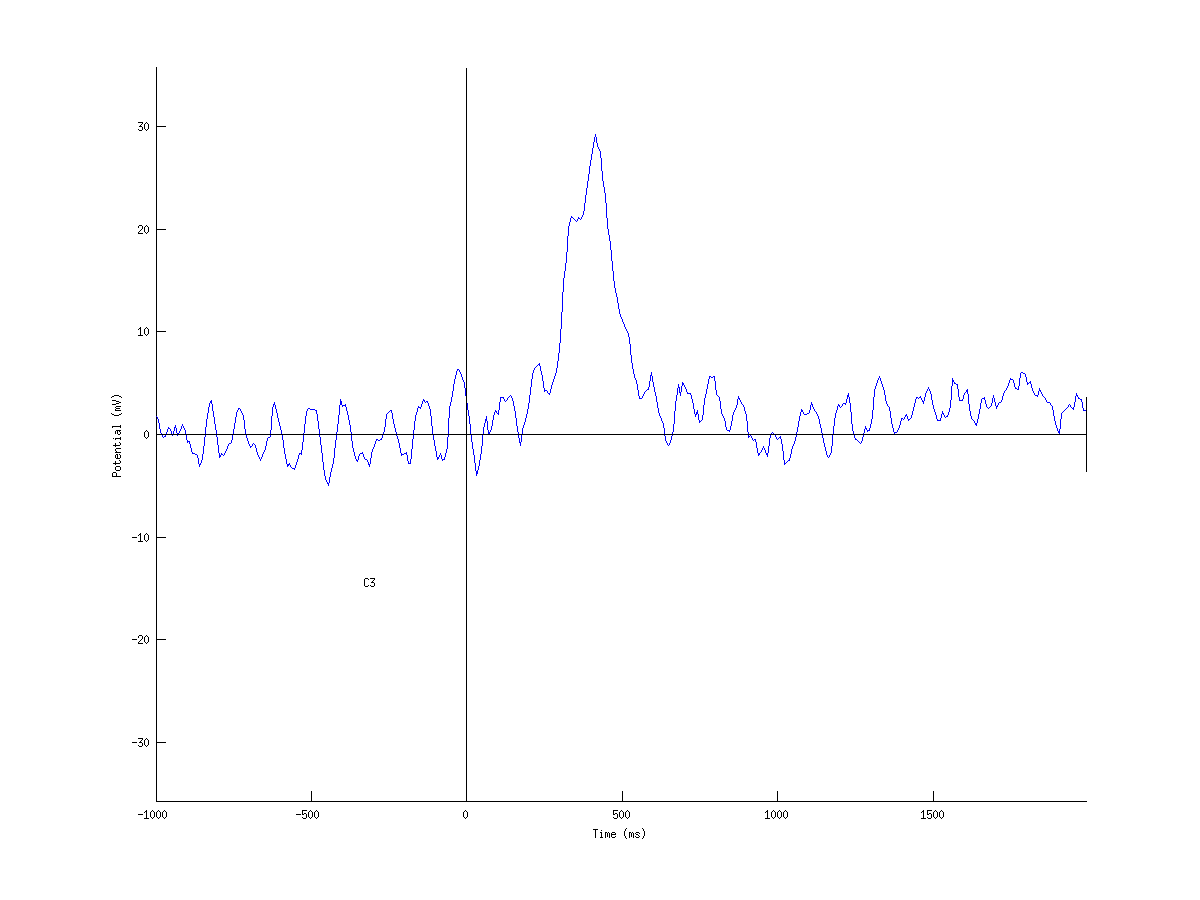
\includegraphics[scale=0.5]{C3.png}
        \caption{Expected waveform for \emph{C3}}
    \end{center}
\end{figure}
\begin{figure}
    \begin{center}
        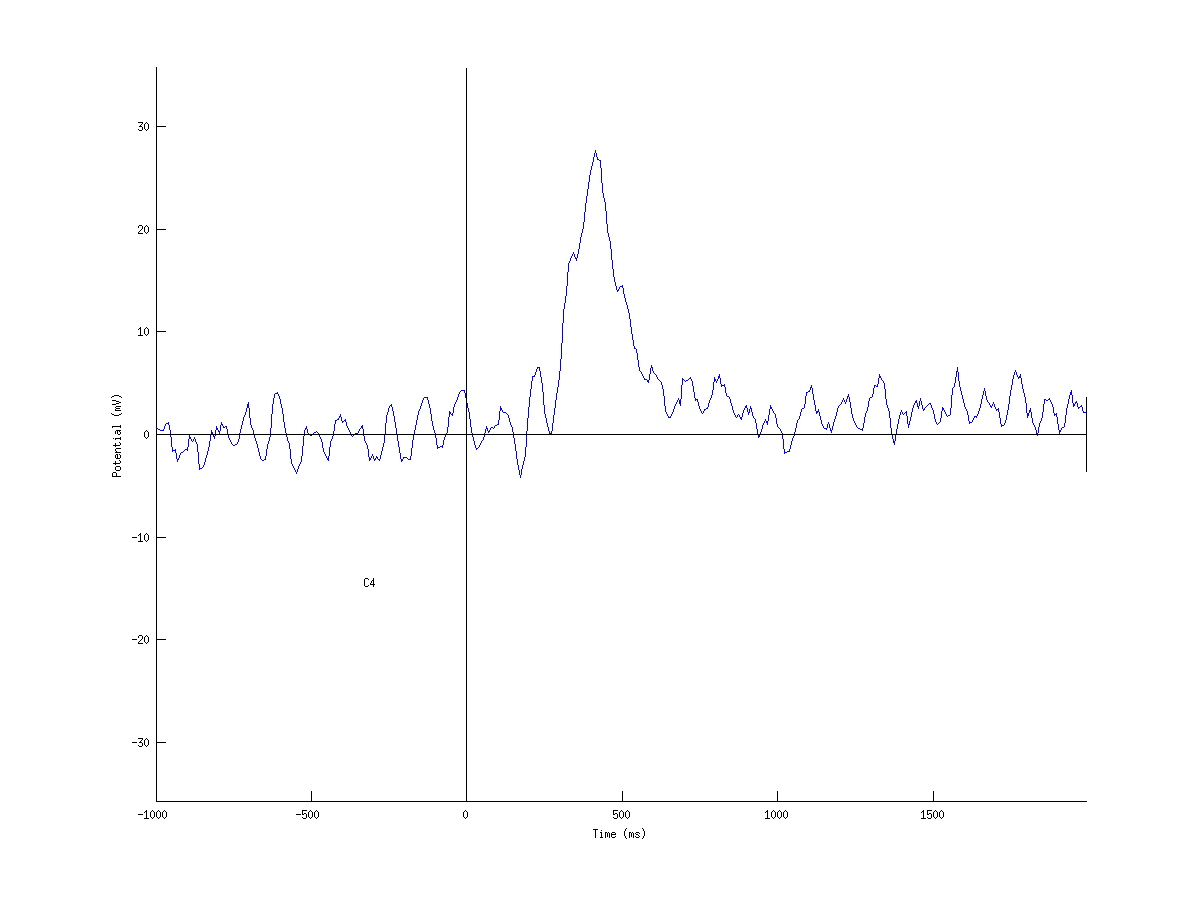
\includegraphics[scale=0.5]{C4.png}
        \caption{Expected waveform for \emph{C4}}
    \end{center}
\end{figure}

\subsection{Equations}
The equations for my model is fairly straight-forward: \[\nabla\cdot(-\sigma\nabla V)=0\]

To calculate each of the lead-fields due to 8 pairs of electrodes (out of five total), we use this equation, and the boundary conditions:
\begin{itemize}
    \item No flux conditions everywhere except for at the electrodes.
    \item The magnitude injected and sunk for each pair of electrodes is 1mA.
    \item Set the potential at the surface at the mid-point between the two electrodes for that given calculation to 0.
\end{itemize}

With the lead-fields calculated, we can then use the reciprocity theorem to calculate the source dipole moments:
\[V_{ab}=\int_V \mathbf{J_i}\cdot\nabla\phi_2 dv\]
,where $V_{ab}$ is the difference between the ERPs measured at electrodes $a$ and $b$, $\phi_2$ is the lead-potential due to that pair of electrodes inside the brain. We are then solving the inverse problem for the components of $\mathbf{J_i}$, which are the source dipole moments.


\begin{thebibliography}{3}
        \bibitem{RushDriscoll1}
            Rush, S.; Driscoll, D. A.; ``Current distribution in the brain from surface electrodes'', \emph{Anesthesia and Analgesia}, vol. 47, pp. 717-723, Nov-Dec 1968.
        \bibitem{RushDriscoll2}
             Rush, S.; Driscoll, D. A.; ``EEG electrode sensitivity - an application of reciprocity'', \emph{IEE Trans on Bio-medical Eng}, vol. BME-16, pp. 15-22, Jan 1969.
        \bibitem{HanzReview}
            Hallez, H et al. ``Review on Solving the Forward Problem in EEG Source Analysis'', \emph{Journal of NeuroEngineering and Rehabilitation}, 2007.
        \bibitem{3dipole}
            Turetsky, B.; Raz, J.; Fein, G; ``Representation of multi-channel evoked potential data using a dipole component model of intracranial generators: application to the auditory P300'', \emph{Electroencephalography and Clinical Neurophys}, vol. 76, pp. 540-556, Dec 1990.
        \bibitem{EEGLab}
            Delorme, A.; Makeig, S.; ``EEGLAB: an open source toolbox for analysis of single-trial EEG dynamics including independent component analysis'', \emph{Journal of Neuroscience Methods}, Vol. 134, Issue 1, pp. 9-21, Mar 2004.
        \bibitem{EEGSource}
        Makeig, S.; Westerfield, M.; Jung, T.P.; Covington, J.; Townsend, J; Sejnowiski T.J.; Courchesne, E; ``Functionally independent components of the late positive event-related potential during visual spatial attention'', \emph{J. Neurosci}, Vol.19, pp. 2665-2680, 1999.

\end{thebibliography}


\end{document}
